
\documentclass[letterpaper,hide notes,xcolor={table,svgnames},pdftex]{beamer}
\def\showexamples{t}


%\usepackage[svgnames]{xcolor}

%% Demo talk
%\documentclass[letterpaper,notes=show]{beamer}

\usecolortheme{crane}
\setbeamertemplate{navigation symbols}{}

\usetheme{MyPittsburgh}
%\usetheme{Frankfurt}

%\usepackage{tipa}

\usepackage{hyperref}
\usepackage{graphicx,xspace}
\usepackage[normalem]{ulem}

\newcommand\SF[1]{$\bigstar$\footnote{SF: #1}}



\newcounter{tmpnumSlide}
\newcounter{tmpnumNote}

% old question code
%\newcommand\question[1]{{$\bigstar$ \small \onlySlide{2}{#1}}}
% \newcommand\nquestion[1]{\ifdefined \presentationonly \textcircled{?} \fi \note{\par{\Large \textbf{?}} #1}}
% \newcommand\nanswer[1]{\note{\par{\Large \textbf{A}} #1}}


 \newcommand\mnote[1]{%
   \addtocounter{tmpnumSlide}{1}
   \ifdefined\showcues {~\tiny\fbox{\arabic{tmpnumSlide}}}\fi
   \note{\setlength{\parskip}{1ex}\addtocounter{tmpnumNote}{1}\textbf{\Large \arabic{tmpnumNote}:} {#1\par}}}

\newcommand\mmnote[1]{\note{\setlength{\parskip}{1ex}#1\par}}

%\newcommand\mnote[2][]{\ifdefined\handoutwithnotes {~\tiny\fbox{#1}}\fi
% \note{\setlength{\parskip}{1ex}\textbf{\Large #1:} #2\par}}

%\newcommand\mnote[2][]{{\tiny\fbox{#1}} \note{\setlength{\parskip}{1ex}\textbf{\Large #1:} #2\par}}

\newcommand\mquestion[2]{{~\color{red}\fbox{?}}\note{\setlength{\parskip}{1ex}\par{\Large \textbf{?}} #1} \note{\setlength{\parskip}{1ex}\par{\Large \textbf{A}} #2\par}\ifdefined \presentationonly \pause \fi}

\newcommand\blackboard[1]{%
\ifdefined   \showblackboard
  {#1}
  \else {\begin{center} \fbox{\colorbox{blue!30}{%
         \begin{minipage}{.95\linewidth}%
           \hspace{\stretch{1}} Some space intentionally left blank; done at the blackboard.%
         \end{minipage}}}\end{center}}%
         \fi%
}



%\newcommand\q{\tikz \node[thick,color=black,shape=circle]{?};}
%\newcommand\q{\ifdefined \presentationonly \textcircled{?} \fi}

\usepackage{listings}
\lstset{%
  keywordstyle=\bfseries,
  aboveskip=15pt,
  belowskip=15pt,
  captionpos=b,
  identifierstyle=\ttfamily,
  escapeinside={(*@}{@*)},
  stringstyle=\ttfamiliy,
  frame=lines,
  numbers=left, basicstyle=\scriptsize, numberstyle=\tiny, stepnumber=0, numbersep=2pt}

\usepackage{siunitx}
\newcommand\sius[1]{\num[group-separator = {,}]{#1}\si{\micro\second}}
\newcommand\sims[1]{\num[group-separator = {,}]{#1}\si{\milli\second}}
\newcommand\sins[1]{\num[group-separator = {,}]{#1}\si{\nano\second}}
\sisetup{group-separator = {,}, group-digits = true}

%% -------------------- tikz --------------------
\usepackage{tikz}
\usetikzlibrary{positioning}
\usetikzlibrary{arrows,backgrounds,automata,decorations.shapes,decorations.pathmorphing,decorations.markings,decorations.text}

\tikzstyle{place}=[circle,draw=blue!50,fill=blue!20,thick, inner sep=0pt,minimum size=6mm]
\tikzstyle{transition}=[rectangle,draw=black!50,fill=black!20,thick, inner sep=0pt,minimum size=4mm]

\tikzstyle{block}=[rectangle,draw=black, thick, inner sep=5pt]
\tikzstyle{bullet}=[circle,draw=black, fill=black, thin, inner sep=2pt]

\tikzstyle{pre}=[<-,shorten <=1pt,>=stealth',semithick]
\tikzstyle{post}=[->,shorten >=1pt,>=stealth',semithick]
\tikzstyle{bi}=[<->,shorten >=1pt,shorten <=1pt, >=stealth',semithick]

\tikzstyle{mut}=[-,>=stealth',semithick]

\tikzstyle{treereset}=[dashed,->, shorten >=1pt,>=stealth',thin]

\usepackage{ifmtarg}
\usepackage{xifthen}
\makeatletter
% new counter to now which frame it is within the sequence
\newcounter{multiframecounter}
% initialize buffer for previously used frame title
\gdef\lastframetitle{\textit{undefined}}
% new environment for a multi-frame
\newenvironment{multiframe}[1][]{%
\ifthenelse{\isempty{#1}}{%
% if no frame title was set via optional parameter,
% only increase sequence counter by 1
\addtocounter{multiframecounter}{1}%
}{%
% new frame title has been provided, thus
% reset sequence counter to 1 and buffer frame title for later use
\setcounter{multiframecounter}{1}%
\gdef\lastframetitle{#1}%
}%
% start conventional frame environment and
% automatically set frame title followed by sequence counter
\begin{frame}%
\frametitle{\lastframetitle~{\normalfont(\arabic{multiframecounter})}}%
}{%
\end{frame}%
}
\makeatother

\makeatletter
\newdimen\tu@tmpa%
\newdimen\ydiffl%
\newdimen\xdiffl%
\newcommand\ydiff[2]{%
    \coordinate (tmpnamea) at (#1);%
    \coordinate (tmpnameb) at (#2);%
    \pgfextracty{\tu@tmpa}{\pgfpointanchor{tmpnamea}{center}}%
    \pgfextracty{\ydiffl}{\pgfpointanchor{tmpnameb}{center}}%
    \advance\ydiffl by -\tu@tmpa%
}
\newcommand\xdiff[2]{%
    \coordinate (tmpnamea) at (#1);%
    \coordinate (tmpnameb) at (#2);%
    \pgfextractx{\tu@tmpa}{\pgfpointanchor{tmpnamea}{center}}%
    \pgfextractx{\xdiffl}{\pgfpointanchor{tmpnameb}{center}}%
    \advance\xdiffl by -\tu@tmpa%
}
\makeatother
\newcommand{\copyrightbox}[3][r]{%
\begin{tikzpicture}%
\node[inner sep=0pt,minimum size=2em](ciimage){#2};
\usefont{OT1}{phv}{n}{n}\fontsize{4}{4}\selectfont
\ydiff{ciimage.south}{ciimage.north}
\xdiff{ciimage.west}{ciimage.east}
\ifthenelse{\equal{#1}{r}}{%
\node[inner sep=0pt,right=1ex of ciimage.south east,anchor=north west,rotate=90]%
{\raggedleft\color{black!50}\parbox{\the\ydiffl}{\raggedright{}#3}};%
}{%
\ifthenelse{\equal{#1}{l}}{%
\node[inner sep=0pt,right=1ex of ciimage.south west,anchor=south west,rotate=90]%
{\raggedleft\color{black!50}\parbox{\the\ydiffl}{\raggedright{}#3}};%
}{%
\node[inner sep=0pt,below=1ex of ciimage.south west,anchor=north west]%
{\raggedleft\color{black!50}\parbox{\the\xdiffl}{\raggedright{}#3}};%
}
}
\end{tikzpicture}
}


%% --------------------

%\usepackage[excludeor]{everyhook}
%\PushPreHook{par}{\setbox0=\lastbox\llap{MUH}}\box0}

%\vspace*{\stretch{1}

%\setbox0=\lastbox \llap{\textbullet\enskip}\box0}

\setlength{\parskip}{\fill}

\newcommand\noskips{\setlength{\parskip}{1ex}}
\newcommand\doskips{\setlength{\parskip}{\fill}}

\newcommand\xx{\par\vspace*{\stretch{1}}\par}
\newcommand\xxs{\par\vspace*{2ex}\par}
\newcommand\tuple[1]{\langle #1 \rangle}
\newcommand\code[1]{{\sf \footnotesize #1}}
\newcommand\ex[1]{\uline{Example:} \ifdefined \presentationonly \pause \fi
  \ifdefined\showexamples#1\xspace\else{\uline{\hspace*{2cm}}}\fi}

\newcommand\ceil[1]{\lceil #1 \rceil}


\AtBeginSection[]
{
   \begin{frame}
       \frametitle{Outline}
       \tableofcontents[currentsection]
   \end{frame}
}



\pgfdeclarelayer{edgelayer}
\pgfdeclarelayer{nodelayer}
\pgfsetlayers{edgelayer,nodelayer,main}

\tikzstyle{none}=[inner sep=0pt]
\tikzstyle{rn}=[circle,fill=Red,draw=Black,line width=0.8 pt]
\tikzstyle{gn}=[circle,fill=Lime,draw=Black,line width=0.8 pt]
\tikzstyle{yn}=[circle,fill=Yellow,draw=Black,line width=0.8 pt]
\tikzstyle{empty}=[circle,fill=White,draw=Black]
\tikzstyle{bw} = [rectangle, draw, fill=blue!20, 
    text width=4em, text centered, rounded corners, minimum height=2em]
    
    \newcommand{\CcNote}[1]{% longname
	This work is licensed under the \textit{Creative Commons #1 3.0 License}.%
}
\newcommand{\CcImageBy}[1]{%
	\includegraphics[scale=#1]{creative_commons/cc_by_30.pdf}%
}
\newcommand{\CcImageSa}[1]{%
	\includegraphics[scale=#1]{creative_commons/cc_sa_30.pdf}%
}
\newcommand{\CcImageNc}[1]{%
	\includegraphics[scale=#1]{creative_commons/cc_nc_30.pdf}%
}
\newcommand{\CcGroupBySa}[2]{% zoom, gap
	\CcImageBy{#1}\hspace*{#2}\CcImageNc{#1}\hspace*{#2}\CcImageSa{#1}%
}
\newcommand{\CcLongnameByNcSa}{Attribution-NonCommercial-ShareAlike}

\newenvironment{changemargin}[1]{% 
  \begin{list}{}{% 
    \setlength{\topsep}{0pt}% 
    \setlength{\leftmargin}{#1}% 
    \setlength{\rightmargin}{1em}
    \setlength{\listparindent}{\parindent}% 
    \setlength{\itemindent}{\parindent}% 
    \setlength{\parsep}{\parskip}% 
  }% 
  \item[]}{\end{list}} 




\title{Lecture 14 --- Unified Modelling Language (UML)}

\author{Patrick Lam \& Jeff Zarnett \\ \small \texttt{p.lam@ece.uwaterloo.ca} \& \texttt{jzarnett@uwaterloo.ca}}
\institute{Department of Electrical and Computer Engineering \\[-1ex]
  University of Waterloo}
\date{\today}
\begin{document}

\begin{frame}
  \titlepage
\end{frame}

\begin{frame}
\frametitle{What is UML?}
\begin{changemargin}{1cm}
Unified Modelling Language (UML):

\begin{quote}
specify and document architecture of\\ large object-oriented software systems, \\ using diagrams.
\end{quote}

UML version 2.2 defines  13 diagrams to summarize:\\
 \qquad intended structure (e.g. classes); behaviour; and \\
\qquad interactions of components.
\end{changemargin}
\end{frame}

\begin{frame}
\frametitle{UML Diagrams}
\begin{center}
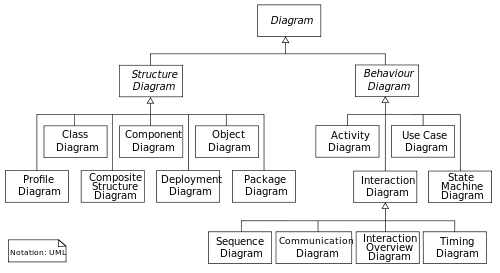
\includegraphics[width=\textwidth]{images/uml-overview}
\end{center}
\end{frame}


\begin{frame}
\frametitle{Why UML}
\begin{changemargin}{1cm}
How much is UML used in industry? Depends where you work.\\
	\quad Some places require it; others forbid it.
	
Standard way to communicate with other programmers.

Mostly, but not only, for Object-Oriented Programming.

\end{changemargin}
\end{frame}



\begin{frame}
\frametitle{Resources}

\begin{changemargin}{1cm}

Lots of information on the Web, e.g. \\
\url{http://edn.embarcadero.com/article/31863}.\\[1em]

Some books:

$\qquad$ Grady Booch, James Rumbaugh, and Ivar Jacobson. \emph{Unified
Modeling Language User Guide,} 2nd Edition, Addison-Wesley, 2005.\\[0.5em]

$\qquad$ Dan Pilone and Neil Pitman. \emph{UML 2.0 in a Nutshell.} O'Reilly Media, 2005.

\end{changemargin}

\end{frame}


\begin{frame}
\frametitle{UML Benefits}

\begin{changemargin}{1cm}
\small
UML is a well-known
language for software designs. In particular, it:

\begin{itemize}
\item is a visual language; UML models are diagrams, so easy
to glance at.
\item models are largely self-documenting.
\item is agnostic in terms of software processes or development lifecycles.
\item is an open standard (not owned by any one company).
\item is good for object-oriented languages, which are quite common.
in industry.
\end{itemize}
\end{changemargin}
\end{frame}

\begin{frame}
\frametitle{Complaints about UML}

\begin{changemargin}{1cm}
Here are some potential complaints about UML.
\begin{itemize}
\item all syntax, no meaning.
\item contains redundant and infrequently-used constructs.
\item complex and difficult to learn.
\item only works for object-oriented languages.
\item tools don't play nicely together.
\end{itemize}
\end{changemargin}
\end{frame}

\begin{frame}
\frametitle{Categories of UML Diagrams}

\begin{changemargin}{1cm}
Three main types:
\begin{itemize}
\item \structure{Structure Diagrams}---static application structure.

\mnote{Examples: class diagrams, object diagrams, component diagrams,
composite structure diagrams, package diagrams, deployment diagrams.\\[1em]}

\item \structure{Behaviour Diagrams}---usage of components,
 activity of components, and finite-state machines summarizing components'
states.

\mnote{$\qquad$ Examples: use case diagrams, activity diagrams, state machine diagrams.\\[1em]}

\item \structure{Interaction Diagrams}---how do components interact?:
  Communication and synchronization, potentially timed.  

\mnote{$\qquad$ Examples: sequence diagrams, communication diagrams, timing diagrams,
and interaction overview diagrams.}
\end{itemize}
\end{changemargin}
\end{frame}

\begin{frame}
\frametitle{Tool Support}

\begin{changemargin}{1cm}
Software tools can create UML diagrams.\\
\qquad e.g. Microsoft Visio, {\tt dia}.\\[1em]

Tools can generate
code from UML and UML from code.\\
\structure{Round-tripping}: going both ways.\\[1em]

Tools can also (sort of) generate test cases and test suites from UML
diagrams.
\end{changemargin}
\end{frame}


\part{UML Class Diagrams}
\frame{\partpage}


\begin{frame}
\frametitle{About Class Diagrams}

\begin{changemargin}{1cm}
The basic UML diagram.\\[1em]

Describes the members of a class:
\begin{itemize}
\item attributes/fields;
\item operations (constructors,
destructors, methods, indexers, and properties).
\end{itemize}
\end{changemargin}
\end{frame}

\begin{frame}
\frametitle{Basic Class Diagram Example; Visibility Symbols}

\begin{changemargin}{1cm}
\begin{center}
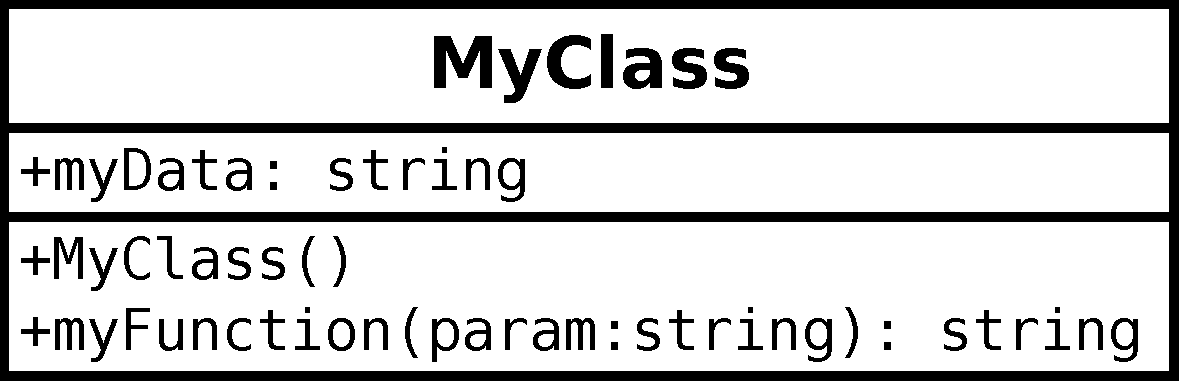
\includegraphics[width=.6\textwidth]{images/myclass.pdf}
\end{center}
~\\[1em]
\begin{itemize}
\item A {\tt +} (plus sign) = public visibility (seen above).
\item A {\tt -} (minus sign) = private visibility.
\item A {\tt \#} (hash sign) = protected visibility.
\end{itemize}

\end{changemargin}
\end{frame}

\begin{frame}
\frametitle{Other UML Symbols}

\begin{changemargin}{1cm}
UML also uses the following symbols:
\begin{itemize}
\item A {\tt $\sim$} (tilde) indicates a destructor (in front of an operation) 
or package (as a visibility symbol).
\item An {\tt ..} (ellipsis) indicates a range of values.
\item A {\tt :} (colon) separates a name from a type.
\item A {\tt ,} (comma) separates items in a set.
\end{itemize}
\end{changemargin}
\end{frame}

\begin{frame}[fragile]
\frametitle{Another UML Class Diagram}

\begin{changemargin}{1cm}

\begin{center}
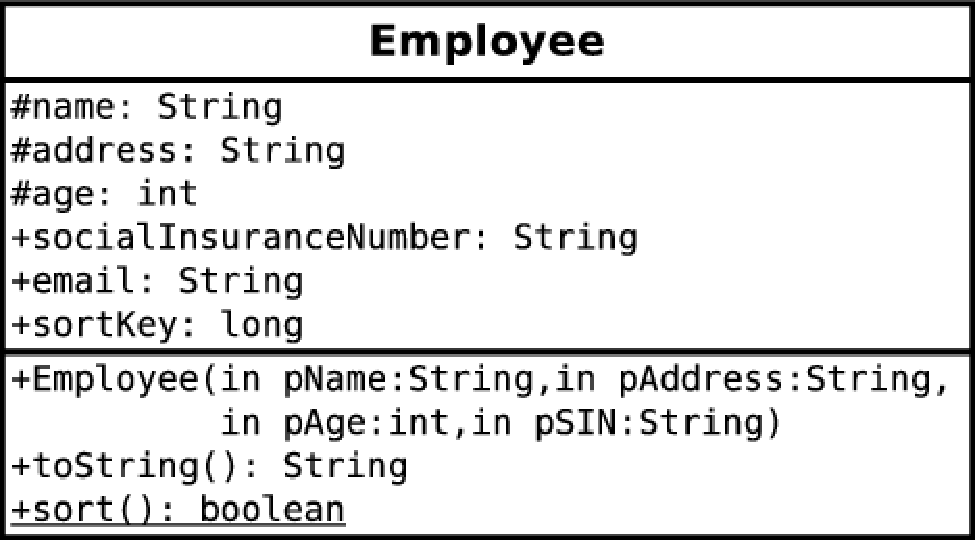
\includegraphics[height=8em]{images/Employee.pdf}
\end{center}

\begin{lstlisting}[language={Java},basicstyle=\tiny]
class Employee {
  protected String name;
  protected String address;
  protected int age;
  public String socialInsuranceNumber;
  public String email;
  public long sortKey;

  public Employee(String pName, String pAddress, 
                  int pAge, String pSIN) { /* ... */ }
  @Override public String toString() { /* ... */ }
  public static boolean sort() { /* ... */ }
}
\end{lstlisting}
\end{changemargin}
\end{frame}

\begin{frame}
\frametitle{Class Hierarchies in UML}

\begin{changemargin}{1cm}
UML represents relationships
between classes and instances.

Between instances of classes:
\begin{itemize}
\item \structure{association}: a relationship between instances
of 2 classes.
\item \structure{aggregation}: a type of association, typically between a
collection or container instance and contents.
\item \structure{composition}: another type of association, typically
between a container and its contents. \\
For a composition, the contents
don't make any sense if the container isn't around.
\end{itemize}

But: a \structure{generalization} relates base classes (not
instances) and their derived classes.
\end{changemargin}
\end{frame}

\begin{frame}
\frametitle{Associations: ``has-a'' links between classes}

\begin{changemargin}{1cm}
Typically one of the
classes can call methods on the other.
\begin{center}

\includegraphics[width=.5\textwidth]{images/association.pdf}
\end{center}

\begin{itemize}
\item Instructors and courses are associated, but there is no subtype
relationship, and the types aren't collection types. 

\item Instructors
teach between 0 and 3 courses per term. 

\item Each course has at least 1
instructor. \mnote{but possibly an unlimited number.}

\item A method that the
instructor might call on the course might be {\tt giveLecture()}.
\end{itemize}
\end{changemargin}
\end{frame}

\begin{frame}
\frametitle{Aggregations}

\begin{changemargin}{1cm}
Specialized
types of associations; \\
also represent ``has-a'' relationships, but
more ``part-whole'' relationships.
\begin{center}
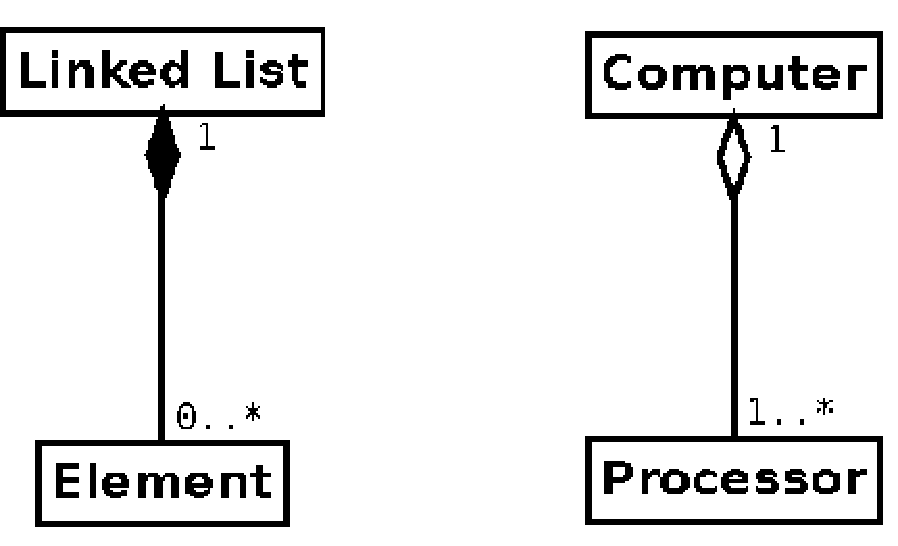
\includegraphics[height=7em]{images/aggr-comp.pdf}
\end{center}
Linked List contains 0 or more Elements.\\
Elements belong to only
one Linked List.\\[1em]

Composition means that we are
saying that Elements may not exist independently of a Linked List.
\end{changemargin}
\end{frame}

\begin{frame}
\frametitle{Compositions}

\begin{changemargin}{1cm}
\begin{center}
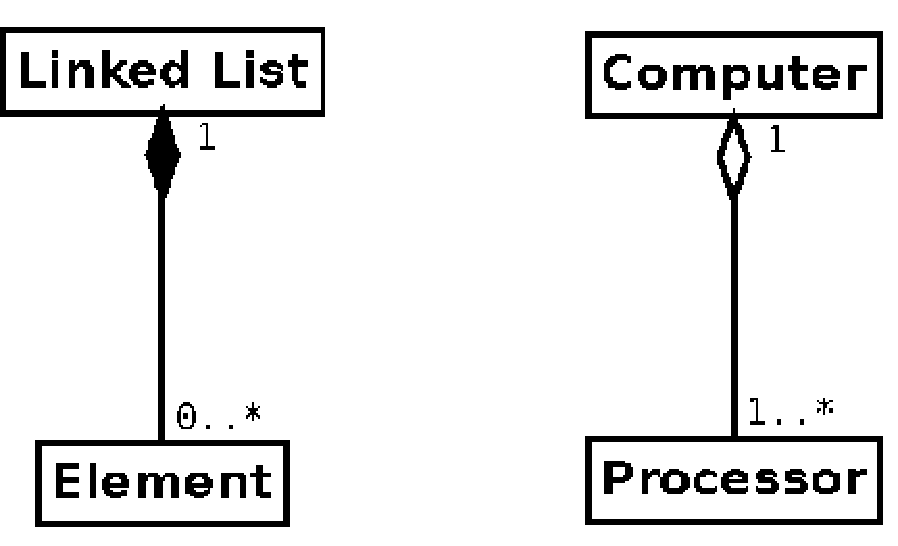
\includegraphics[height=7em]{images/aggr-comp.pdf}
\end{center}
Computers contain 1 or more Processors, but \\
Processors only
belong to 1 Computer. \\[1em]

In an aggregation, we are stating that 
Processors do exist independently of a Computer.
\end{changemargin}
\end{frame}

\begin{frame}
\frametitle{Generalizations}

\begin{changemargin}{1cm}
Relationships between
classes.\\[1em]
\begin{center}
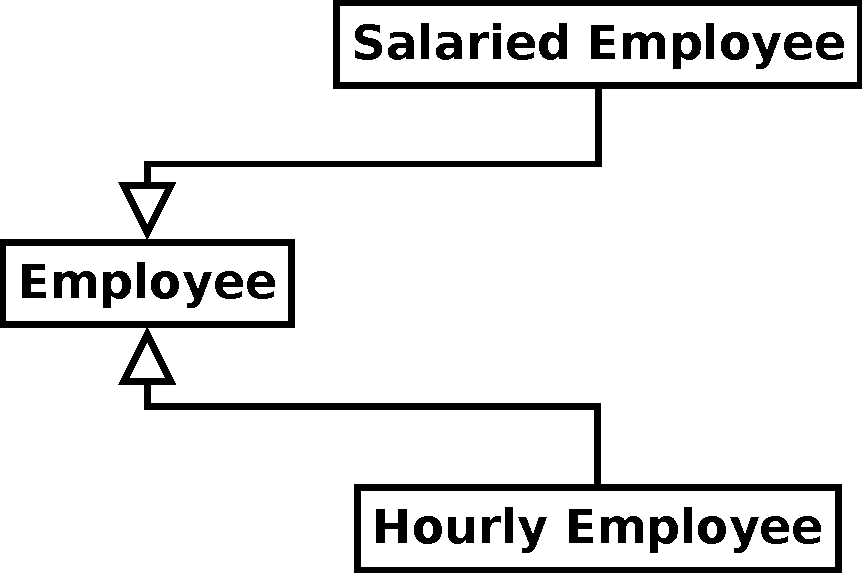
\includegraphics[width=.3\textwidth]{images/generalization.pdf}
\end{center}
\small
Every Salaried Employee and Hourly Employee is an Employee, \\
so Employees are generalizations of the Salaried and Hourly
Employee classes.\\[1em]

 In code: Salaried Employee
and Hourly Employee would be subclasses of (``extend'') Employee.
\end{changemargin}
\end{frame}

\begin{frame}
\frametitle{More Class Diagrams I}

\begin{changemargin}{1cm}

From \url{http://www.altova.com/umodel/class-diagrams.html}
(accessed March 10, 2011).:

\begin{center}
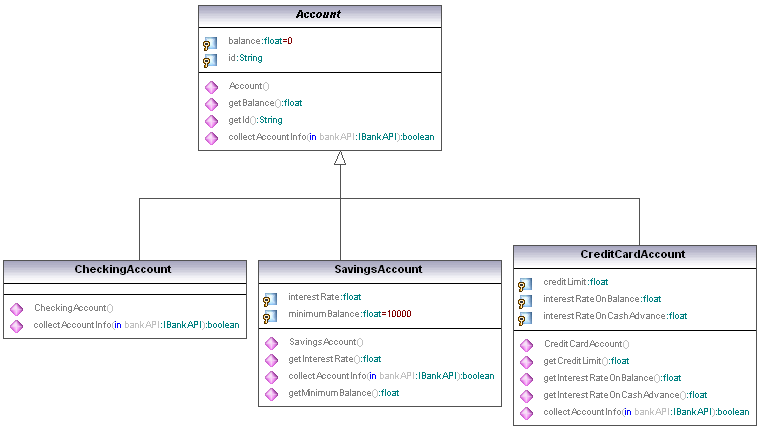
\includegraphics[width=.8\textwidth]{images/UML_class_diagram_example.png}
\end{center}
Note the member field initializations and the generalization link.

\end{changemargin}
\end{frame}


\begin{frame}
\frametitle{More Class Diagrams II}

\begin{changemargin}{1cm}
From \url{http://edn.embarcadero.com/article/31863} (accessed March 10, 2011).
\begin{center}
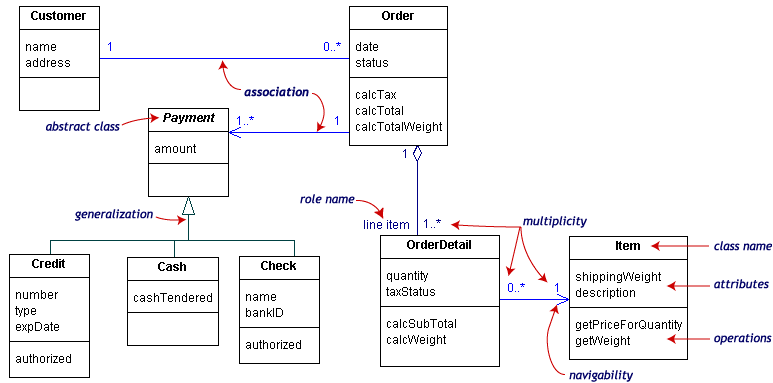
\includegraphics[width=.8\textwidth]{images/classdiagramno3d.png}
\end{center}

\end{changemargin}
\end{frame}


\begin{frame}

\frametitle{State Diagrams: Learning Outcome} 

\begin{changemargin}{1cm}

You should be able to:
\begin{itemize}
\item read a description of
a finite state machine (either in code or in text) and produce a
syntactically correct UML state diagram summarizing that design.
\end{itemize}

(Examples are from \emph{UML Distilled, Second
  Edition}, by Martin Fowler with Kendall Scott.)
\end{changemargin}

\end{frame}

\begin{frame}

\frametitle{UML State Diagram: Order Processing System}


\begin{center}
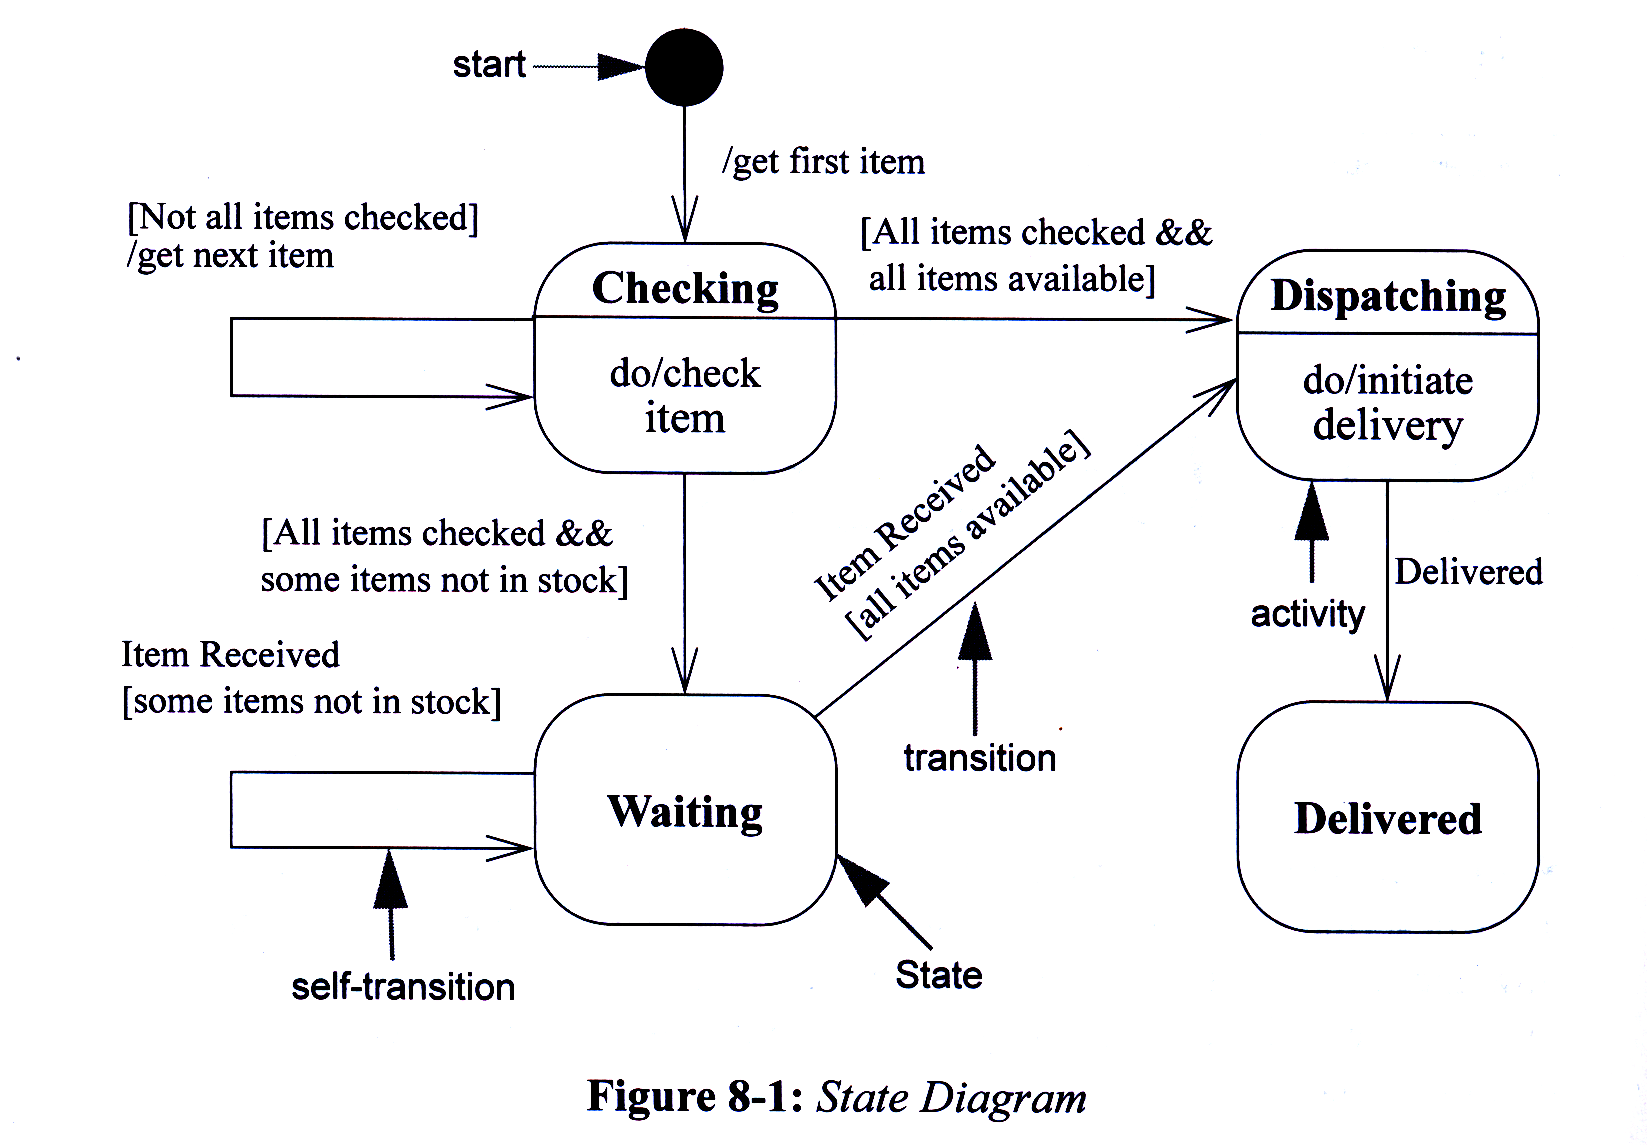
\includegraphics[width=0.7\textwidth]{images/statediagram1}
\end{center} \mnote{Note: lots of time spent explaining how to read and understand the state diagram}

\end{frame}

\begin{frame}
\frametitle{UML State Diagram: States}

\begin{changemargin}{1cm}

Example: states of an order 
in an order processing system. \\

Order object has 4 states, represented by boxes.\\[1em]

Upper half of
the box = name,\\
\quad e.g. ``checking'', ``dispatching'', ``waiting'', ``delivered''.\\

Lower half = what the activity in that state is.\\[1em]

 ``Dispatching'' state initiates the delivery of the
order. \\[1em]

In ECE155, you can always put ``do'' before the slash
and the activity after the slash.\\[1em]

State have names and may have activities. \\
Objects carry out activities, and these activities take some amount of time.
\end{changemargin}
\end{frame}

\begin{frame}
\frametitle{UML State Diagram: Transitions}

\begin{changemargin}{1cm}
Edges = transitions between states,
optionally labelled.\\

Three parts
to a transition label: \emph{Event [Guard] / Action}.\\[1em]
\alert{An object takes transition if event occurs and guard is true.}\\

Example: self-transition from  ``checking''
contains  guard ``[not all items checked]'' and performs
 action ``get next item''. \\[1em]

\structure{Event}: something happening to an object, e.g. ``Item
Received''.  \\

\structure{Guard}: logical condition that states the conditions
under which the event may occur (e.g. ``[some items not in stock]'').\\[1em]

Objects carry out \structure{actions}, e.g. ``get next
item''.\\
Actions must occur quickly and be uninterruptible.\\[1em]

% (contrast
%this with an activity, which takes longer and gets interrupted by
%events).

%Before machine completes the transition and enters the destination, it
%carries out action.\\

UML state machines are deterministic: at most one
transition should be activated at once.

\end{changemargin}
\end{frame}

\begin{frame}
\frametitle{UML State Diagram: Superstates}

\begin{changemargin}{1cm}

State diagrams may get too complicated.\\[1em]

UML's solution: hierarchical nesting:
\begin{itemize}
\item can help write clearer diagrams;
\item allow understanding system's higher-level structure.
\end{itemize}~\\

Concept: \structure{superstate}.

\begin{itemize}
\item  may contain nested states and transitions;\\
 make up a state machine for some subset of the entire machine's behaviour.
\end{itemize}

\end{changemargin}
\end{frame}

\begin{frame}
\frametitle{UML State Diagram: Superstate Example}

\begin{center}
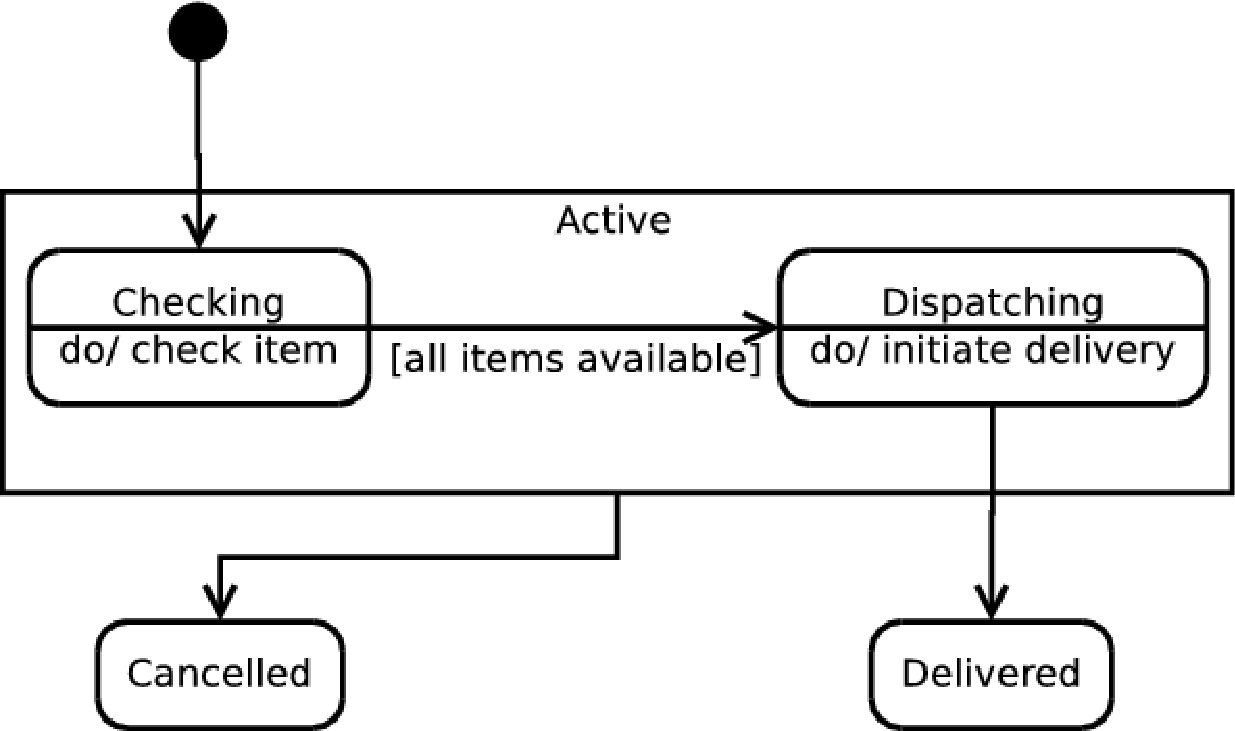
\includegraphics[width=.5\textwidth]{images/statediagram2.pdf}

\scriptsize (\tiny\url{http://atlas.kennesaw.edu/~dbraun/csis4650/A&D/UML_tutorial/state.htm}. Accessed July 3, 2011.)
\end{center}

\begin{changemargin}{1cm}
Superstate ``active'' contains ``checking'' and ``dispatching''.\\[0.5em]

Note transitions from states inside
superstate,\\
 e.g. ``dispatching'' to ``delivered'', \\ plus transition
from the superstate to the ``cancelled'' state. \\

So, either of the states in the superstate can get to ``cancelled''. \\[0.5em]

Superstate transition = transitions from both ``dispatching'' and ``checking''
to ``cancelled''.
\end{changemargin}
\end{frame}

\begin{frame}
\frametitle{UML State Diagram: Timing}

\begin{changemargin}{1cm}

Recall: timing is important for embedded systems.\\[1em]

Your documentation should explain what ``quickly'' \\
\qquad (actions happen quickly) means.\\

UML doesn't say; it depends on the system. \\[1em]

Can also
write an event that happens after some time,\\
\qquad  e.g. ``after (20
minutes)''. 
\end{changemargin}
\end{frame}

\part{UML Use Case Diagrams}
\frame{\partpage}

\begin{frame}
\frametitle{Use cases in UML; actors}

Recall: a use case describes a user's
interaction with a system. \\[1em]

\structure{Actors} represent users (or other systems).

\begin{center}
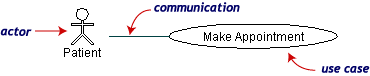
\includegraphics[width=.5\textwidth]{images/usecase-explanation.png}
\end{center}

\end{frame}

\begin{frame}
\frametitle{Example: Multiple actors}

\begin{center}
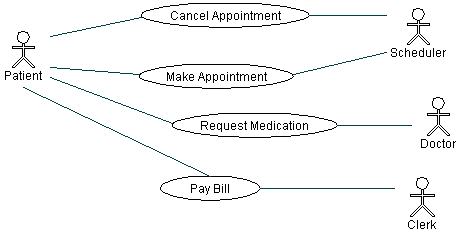
\includegraphics[width=.45\textwidth]{images/usecase-multiple.png}
\end{center}

\begin{changemargin}{1cm}

It's just a coincidence that each use case has two actors.
\end{changemargin}
\end{frame}

\begin{frame}[fragile]
\frametitle{Another use case example}

\begin{center}
\scriptsize \url{http://msdn.microsoft.com/en-us/library/dd409427%28VS.100%29.aspx}
(accessed March 10, 2011).\\[1em]

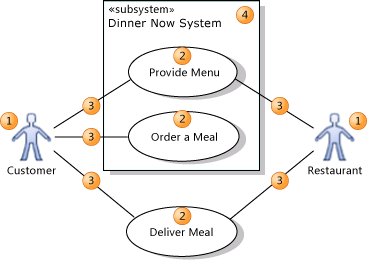
\includegraphics[width=.5\textwidth]{images/dinnernow.png}
\end{center}


\begin{changemargin}{1cm}
Components: 1) actors, 2) use cases, 3) communication, and, new to this
figure, 4) subsystems or components. 
\end{changemargin}

\end{frame}

\begin{frame}
\frametitle{Use cases and actors}

\begin{center}
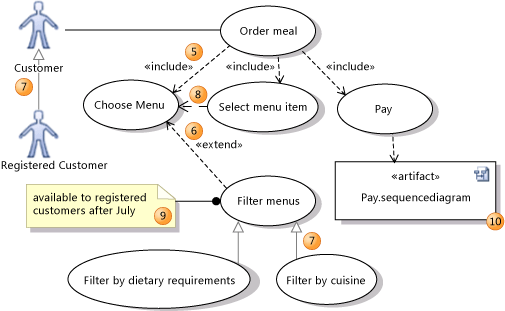
\includegraphics[width=.55\textwidth]{images/dinnernow2.png}
\end{center}

\begin{changemargin}{1cm}

Here we have: 5) inclusion stereotypes on dependencies; 6) extension
stereotypes on dependencies; 7) inheritance relationships between use cases;
8) plain dependencies; 9) comments; and 10) references to other artifacts.

\end{changemargin}
\end{frame}

\begin{frame}
\frametitle{Things in use cases}

\begin{changemargin}{1cm}


\begin{itemize}
\item A \emph{communication} (solid line) represents a relationship
between an actor and a use case.
\item An \emph{inclusion} (dashed line, {\scriptsize$<<$}include{\scriptsize$>>$} ~stereotype)
represents an invocation relationship between use cases; the first use 
case must call the second one.
\item An \emph{extension} (dashed line,{\scriptsize$<<$}extend{\scriptsize$>>$} ~stereotype)
represents an optional invocation of a use case.
\item A \emph{generalization} or \emph{specialization} represents
a case where an actor or use case inherits from another actor or use case.
\end{itemize}
\end{changemargin}
\end{frame}

\begin{frame}
\frametitle{UML use cases: why?}

\begin{changemargin}{1cm}
Can be useful for:
\begin{enumerate}
\item documenting essential features (requirements)\\ of
a software system;
\item communicating system behaviour to clients; 
\item generating appropriate test cases for scenarios.
\end{enumerate}
\end{changemargin}
\end{frame}

\part{UML Sequence Diagrams}
\frame{\partpage}

\begin{frame}
\frametitle{About UML Sequence Diagrams}

\begin{changemargin}{1cm}

UML sequence diagrams:
\end{changemargin}
\begin{quote}
 express system behaviour as a sequence
of events and activities.
\end{quote}

\begin{changemargin}{1cm}
Things you'll find: \\
objects, lifelines, messages,
action boxes, and gates.
\end{changemargin}
\end{frame}

\begin{frame}
\frametitle{Elements in UML Sequence Diagrams}

\begin{changemargin}{1cm}

\begin{itemize}
\item \structure{Instances} of objects: boxes at the top of the diagram.
\item \structure{Lifelines} (vertical dashed lines, extending
downwards from instances of the objects): denote the passing of time.
\item \structure{Messages} (horizontal lines): denote 
communication between objects.
\item \structure{Action boxes} (boxes on top of lifelines): denote
the occurrence of activities.
\item \structure{Gates} (filled circles on the boundary of the diagram):
denote occurrence of external events.
\end{itemize}

\end{changemargin}
\end{frame}

\begin{frame}
\frametitle{Sequence diagram, financial reporting system}

\begin{center}
\scriptsize (IBM, \emph{UML basics: The sequence
  diagram},
\url{http://www.ibm.com/developerworks/rational/library/3101.html},
accessed March 10, 2011).

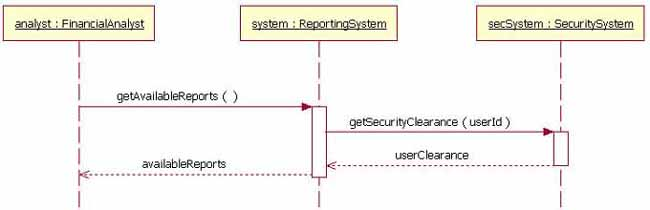
\includegraphics[width=0.7\textwidth]{images/uml_sequence.png}
\end{center}

\begin{changemargin}{1cm}
Solid lines are initiating messages.

Dashed lines are responses.\\[0.5em]

Also: synchronous messages (solid arrowhead---all initiating
messages in the above example) \\
and asynchronous messages (stick
arrowhead---responses).\\[0.5em]

You can also use: actors, destroy elements, scenario elements, timer elements.
\end{changemargin}

\end{frame}

\begin{frame}
\frametitle{Sequence diagram, student records}

\begin{changemargin}{1cm}
\begin{center}
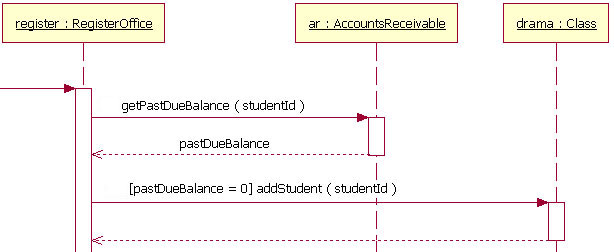
\includegraphics[width=0.7\textwidth]{images/student_records.png}
\end{center}
Note guards on messages; must be satisfied before
the message gets sent.\\

\end{changemargin}
\end{frame}

\begin{frame}
\frametitle{Sequence diagram: when?}

\begin{changemargin}{1cm}
UML sequence
diagrams help document messages going between different instances of
objects, \\ including the ordering in which these events occur  (for synchronous events).\\[1em]

Exercise judgment to include the right level of detail.\\
\begin{itemize}
\item too much detail makes the model difficult to
understand;
\item too little detail doesn't document anything.
\end{itemize}

You can use more than one UML sequence diagram to document a large system.
\end{changemargin}
\end{frame}





\end{document}
